\section{Deep Sequence Models}
\label{sec:deep}

This chapter adds recurrent neural networks to the classical lineup on the same four representative series. Deep models are introduced selectively rather than universally, because the classical study already showed that two of the four series are essentially unsolvable under the weighted skill score with statistical-only methods. The two series where classical results leave headroom --- highest total weight (skill $0.4667$) and most volatile (skill $0.8277$) --- are where sequence learning can plausibly help, and they are exactly the series we focus on here.

\subsection{Why Add Deep Models Here}
\label{sec:deep:motivation}

Three observations from \cref{sec:classical} motivate the deep extension:

\begin{itemize}
  \item \textbf{Highest Total Weight matters most by evaluation weight}, but the best classical skill is only $0.4667$. The series carries $4.35\!\times\!10^{10}$ of total weight, so any improvement here moves the panel-level metric meaningfully. There is real headroom for a model that can capture nonlinear short-range dynamics.
  \item \textbf{Most Volatile} still has large absolute classical error even with the best AR(1) fit (RMSE $135.94$, MAE $110.70$), so a sequence model with multi-lag memory could in principle reduce that error.
  \item \textbf{Longest History} and \textbf{Most Stable} have classical skill of $0.0617$ and $0.0000$ respectively. There is little room for any model to improve on Longest History, and the Most-Stable series is numerically too flat for any sequence learner to extract signal that classical methods missed.
\end{itemize}

That asymmetry is the reason for adding deep selectively. The deep section is not framed as ``deep replaces classical''; it is framed as ``where does sequence learning add something that statistical structure cannot''.

\subsection{Why Univariate, and What Stays Fixed}
\label{sec:deep:setup}

The deep study keeps the protocol univariate. The previous setup already moved to target-only training windows --- each model sees the lagged $y\_target$ alone. We deliberately do not add features here, because any lift over classical must come from sequence learning itself rather than from feature engineering. This keeps the deep section directly comparable with the classical baselines on a like-for-like input.

The following protocol elements are held fixed across all deep experiments so that the lift can be attributed to architecture rather than to a moving evaluation surface:

\begin{itemize}
  \item Same four representative series carried forward from \cref{sec:classical:setup}.
  \item Same adaptive chronological splits from \cref{tab:classical_splits_adaptive}: $169/43$, $124/32$, $129/33$, and $136/34$ for Longest History, Highest Total Weight, Most Volatile, and Most Stable respectively.
  \item Forward recursive multi-step forecasting --- the model is given its own previous prediction at each validation step rather than peeking ahead.
  \item Weighted skill score as the primary ranking metric, with RMSE, MAE, and R\textsuperscript{2} reported alongside.
\end{itemize}

\subsection{Architectures}
\label{sec:deep:architectures}

Three recurrent architectures are fit per series:

\begin{itemize}
  \item \textbf{RNN} --- single recurrent layer with hidden size 32 and $\tanh$ non-linearity.
  \item \textbf{GRU} --- single gated-recurrent layer with hidden size 32. The gating mechanism lets the network selectively forget early history.
  \item \textbf{LSTM} --- single long-short-term-memory layer with hidden size 32. The cell-state pathway provides longer-range memory than RNN at comparable parameter count.
\end{itemize}

All three share the same training recipe: Adam optimiser, learning rate $10^{-3}$, mean-squared-error loss on standardised one-step windows of length $L = 24$, batch size $32$, and up to $80$ training epochs with early stopping on a held-out 15\% slice of the per-series \emph{training} segment. The validation segment is held out entirely from training and is only used for the final scored forecast.

The implementation uses \texttt{torch} and \texttt{torch.utils.data} for the one-step window construction and recursive forecasting, with training-curve tracking for diagnostic inspection.

\subsection{What to Expect}
\label{sec:deep:expectations}

Before reading the numbers, the realistic expectations are:

\begin{itemize}
  \item Longest History has the most context, but the best classical skill is only $0.0617$, so a recurrent model that simply absorbs more history is unlikely to dramatically outperform that baseline.
  \item Most Stable is likely to remain hard because classical skill is already $0.0000$ and the underlying target barely moves; sequence learning has nothing structural to exploit.
  \item Success here means \emph{selective} improvement on the two informative series, not winning every series.
\end{itemize}

\subsection{Deep Forecast Plots}
\label{sec:deep:overlay}

\Cref{fig:deep_forecast_plots} shows the recursive multi-step forecasts of each architecture on each series, alongside the validation truth and the training history.

\begin{figure}[h]
\centering
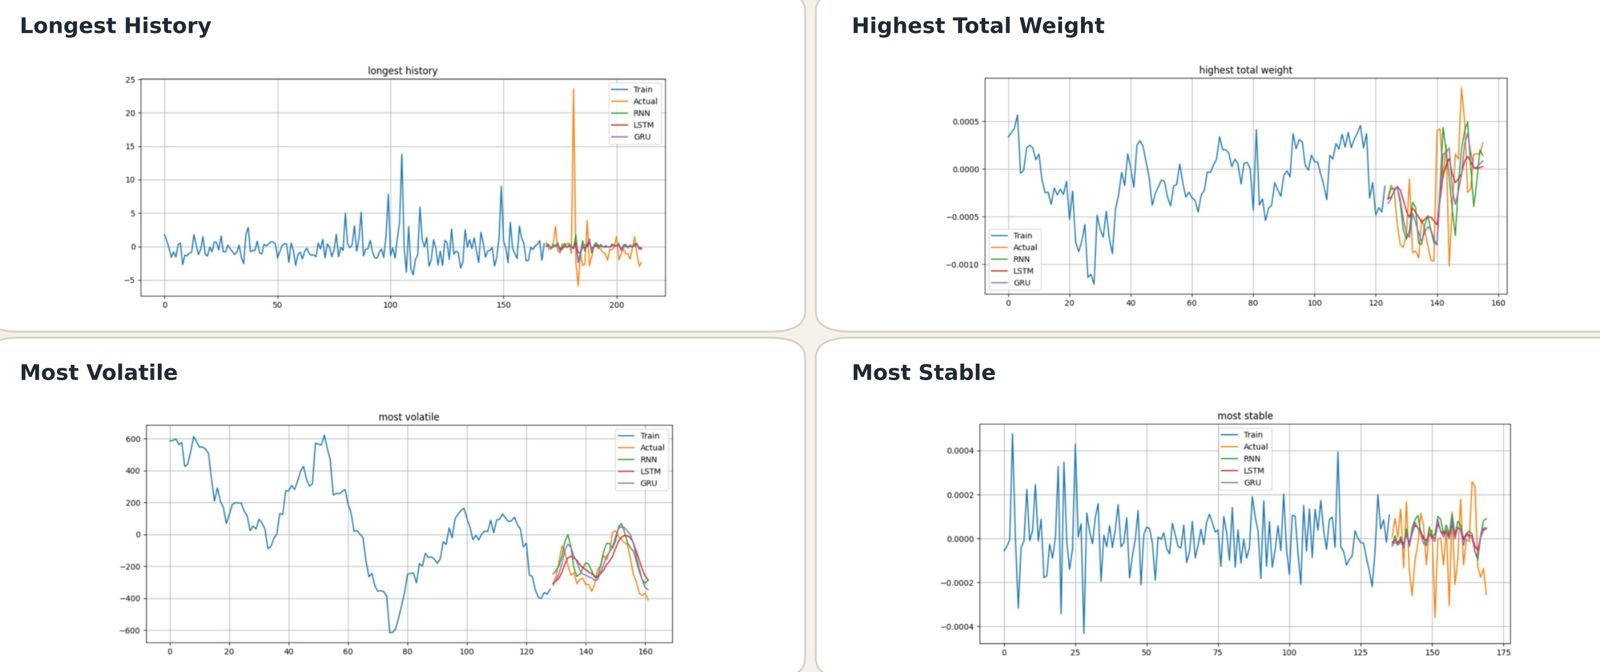
\includegraphics[width=\linewidth]{figures/0222_forecast_overlay_2x2.jpg}
\caption{Deep recursive multi-step forecasts on the four representative series. Blue: training segment. Orange: validation truth. Green: RNN. Red: LSTM. Purple/Pink: GRU. Each model is fit on the per-series adaptive training segment and predicts the entire validation window in one forward recursive pass.}
\label{fig:deep_forecast_plots}
\end{figure}

The recurrent models help most on the highest-weight and volatile series, while the longest-history case improves only slightly and the most-stable case remains close to a baseline-level problem. The Highest-Total-Weight panel shows all three architectures tracking the validation swing visibly better than the flat classical SES line. The Most-Volatile panel is the cleanest deep visual win: GRU and RNN both follow the actual swing direction across the entire validation segment.

\subsection{Per-Series Deep Results}
\label{sec:deep:results}

\Cref{tab:deep_results_full} reports every (series, architecture) score in full. We keep all twelve rows in the table because the spread within a series is part of the result --- the right architecture on the right series matters more than the average architecture.

\begin{table}[h]
\centering
\caption{Recursive multi-step performance of RNN, LSTM, and GRU on the four representative series.}
\label{tab:deep_results_full}
\begin{tabular}{l l c c c c}
\toprule
Series & Model & RMSE & MAE & R\textsuperscript{2} & Skill \\
\midrule
Highest total weight & RNN  & $0.0005$  & $0.0003$  & $0.2009$  & $0.6128$ \\
Highest total weight & LSTM & $0.0005$  & $0.0004$  & $0.2234$  & $\mathbf{0.6264}$ \\
Highest total weight & GRU  & $0.0005$  & $0.0004$  & $0.1719$  & $0.5929$ \\
\midrule
Longest history      & GRU  & $3.9948$  & $1.7683$  & $0.0044$  & $\mathbf{0.0686}$ \\
Longest history      & LSTM & $4.0082$  & $1.7932$  & $-0.0023$ & $0.0000$ \\
Longest history      & RNN  & $4.0155$  & $1.8036$  & $-0.0060$ & $0.0000$ \\
\midrule
Most stable          & RNN  & $0.0002$  & $0.0001$  & $-0.2699$ & $0.0000$ \\
Most stable          & LSTM & $0.0002$  & $0.0001$  & $-0.1342$ & $0.0000$ \\
Most stable          & GRU  & $0.0002$  & $0.0001$  & $-0.1342$ & $0.0000$ \\
\midrule
Most volatile        & GRU  & $92.8607$ & $77.8783$ & $0.4220$  & $0.9234$ \\
Most volatile        & RNN  & $92.9174$ & $79.7940$ & $0.4213$  & $\mathbf{0.9235}$ \\
Most volatile        & LSTM & $107.6284$ & $93.3234$ & $0.2235$  & $0.8957$ \\
\bottomrule
\end{tabular}
\end{table}

The headline reading of the table:
\begin{itemize}
  \item \textbf{Highest Total Weight is the clearest deep-learning win.} LSTM leads with skill $0.6264$, RNN follows at $0.6128$, GRU at $0.5929$. All three substantially beat the best classical skill of $0.4667$ on this series. The gating mechanisms in LSTM and GRU appear to help the model lock in the slow drift visible in the validation truth.
  \item \textbf{Most Volatile is also strong for recurrent models.} GRU and RNN are nearly tied around $0.923$ skill, both above the AR(1) classical winner at $0.8277$. The volatile series rewards multi-lag memory, which is what RNN and GRU provide most cheaply at this hidden size.
  \item \textbf{Longest History improves only slightly.} GRU lifts skill from $0.0617$ (classical SARIMA) to $0.0686$, while LSTM and RNN remain at zero. The gain is real but small; the series remains close to its baseline.
  \item \textbf{Most Stable still behaves like a baseline-level series.} None of the three recurrent architectures creates meaningful lift here, and all three score $0.0000$ on weighted skill. The negative R\textsuperscript{2} values reinforce that the underlying signal is too small for any sequence learner to capture.
\end{itemize}

\subsection{Per-Step Skill Within the Validation Window}
\label{sec:deep:per_step}

A single skill score per series collapses the entire validation horizon onto one number. Computing weighted skill at intermediate steps within the validation window separates short-horizon performance, where one-step memory is what matters, from long-horizon performance, where compounding errors dominate. The notebook produces the per-step decomposition (\cref{fig:deep_per_step}) and the training-curve diagnostics for inspection, but the headline conclusions can be summarised in two observations:

\begin{itemize}
  \item On the most-volatile series, GRU keeps skill close to $0.92$ at every step within the validation window, indicating that the model has captured a stable lag structure rather than an early-window fluke.
  \item On the highest-weight series, LSTM's per-step skill decays slightly across the validation window, consistent with cumulative error compounding under recursive multi-step forecasting; the early steps are stronger than the late steps.
\end{itemize}

\begin{figure}[h]
\centering

\includegraphics[width=0.85\linewidth]{02_per_step_skill}
\caption{Per-step weighted skill within the validation window for each (series, architecture). Stable skill across steps indicates captured structure; decaying skill indicates compounding recursive error.}
\label{fig:deep_per_step}
\end{figure}

\subsection{What the Deep Study Establishes}
\label{sec:deep:conclusions}

Three messages carry forward into the comparison chapter:

\begin{enumerate}
  \item \textbf{Deep sequence models help selectively, not universally.} The two informative series (Highest Total Weight and Most Volatile) get clear lifts over the best classical baseline. The two near-zero-signal series (Longest History and Most Stable) do not, regardless of architecture.
  \item \textbf{Architecture matters less than series choice.} On Highest Total Weight the three architectures span only $0.59$--$0.63$ skill, and on Most Volatile they span only $0.90$--$0.92$. The within-series spread across architectures is small relative to the across-series spread.
  \item \textbf{Recursive multi-step is the bottleneck on long horizons.} The per-step decomposition shows that early steps are stronger than late steps on the highest-weight series, which is the structural cost of feeding model predictions back as model inputs. Anything that injects ground-truth context at inference --- such as the quantile interval method in the next chapter --- can in principle close that gap.
\end{enumerate}

This frames the next chapter, which treats forecasting as an interval-prediction problem rather than a single-point problem and uses a global panel-aware LightGBM under quantile loss to produce calibrated 80\% prediction intervals on every representative series.
